\documentclass[10pt,conference]{IEEEtran}
\usepackage[utf8]{inputenc}
\usepackage{amsmath}
\usepackage{amsfonts}
\usepackage{amssymb}
\usepackage{graphicx}
\usepackage{fixme}
\fxsetup{
    status=final,
    author=Chris,
    layout=margin,
    theme=color,
    targetlayout=color
}

\usepackage[backend=bibtex,style=ieee]{biblatex}
\addbibresource{bib/sdn.bib}
\addbibresource{bib/trust.bib}

%\author{Christopher C. Lamb \\ Department of Electrical and Computer Engineering \\ The University of New Mexico}
%\author{
%\IEEEauthorblockN{Christopher C. Lamb}
%\IEEEauthorblockA{Dept. of Electrical and Computer Engineering\\
%The University of New Mexico\\
%Albuquerque, New Mexico 87131\\
%Email: cclamb@ece.unm.edu}
%\and
%\IEEEauthorblockN{Gregory L. Heileman}
%\IEEEauthorblockA{Dept. of Electrical and Computer Engineering\\
%The University of New Mexico\\
%Albuquerque, New Mexico 87131\\
%Email: heileman@ece.unm.edu}
%}

\title{Towards Robust Trust in Software Defined Networks}
\begin{document}

\maketitle

\begin{abstract}
Software defined networks (SDNs) are becoming more popular in industry, though currently still only deployed by very technically-savvy organizations.  Nevertheless, as the advantages of using SDN become more clear, future adoption promises to be high, with all network equipment vendors quickly moving to deploy products providing SDN capabilities.  This impending wider adoption demands that security implications within SDN be more clearly understood.  Today, mechanisms through which vendors can provide enhanced integrity and availability as well as authentication and non-repudiation are poorly understood and have yet to be thoroughly investigated.  In this paper, we present our current work outlining how we can define trust in SDN and what trust in SDN means for various operational components.  We also address what the operational characteristics that impact trust propagation are, and present promising approaches to managing trust within SDN as an extension of these definitions and attributes.
\end{abstract}

\section{Introduction}
Software Defined Networks (SDNs) are here to stay. The specific technologies are still in question, in that the community has yet to decide if OpenFlow will be the most common southbound protocol, or if it will be supplanted by some other alternative~\cite{rfc6241}.  Nevertheless, intense industry involvement in SDN technologies and techniques makes it clear that organizations will be adopting SDN in the future, whether they would like to or not~\cite{opendaylight}.  In order to effectively deploy SDN systems, we need to have a clear understanding of how we can secure them.  To begin to secure SDN, we need to establish a more general picture of how trust propagates through SDN systems so we can more clearly envision how we can take advantage of hardened or redundant systems to enhance the security posture of deployed systems.  The way we extend trust to components in operational systems is key to defining and clarifying overall security postures in SDN architectures.

This paper represents our work in progress toward defining a rigorous trust model for SDN systems.  As of today, we have framed the problem and defined a general SDN control architectural model over which we will begin to apply mathematical trust models.  This paper will describe this reference model for the SDN control plane, highlight the key attributes of realistic SDN control planes a trust model must handle, and describe promising approaches to mathematically describing trust in SDN.  We close the paper with references to related work and our future plans in this area.

The contributions of this paper are describing the primary components of operational SDN systems, defining the trust relationships that exist and why they are important, outlining why SDN systems differ from other systems with established trust models, and then detailing which approaches to defining SDN trust are most promising and why.

\section{Trust in SDN}
In order to frame the discussion of trust appropriately, we first propose a common model for the SDN control plane.  This model allows us to define the common elements we need to examine, to describe the trust relationships, and describe precisely why these components are forced to trust other elements in the overall trust model.  Here, we are going to limit our taxonomy to objects and classes based on OpenFlow inspired SDNs.

When modern SDN with OpenFlow was first developed, it consisted of a two layers --- a controller layer sending messages to a programmable switching layer.  This provided separation between the control and data forwarding planes, enabling new capabilities for network innovation.  In this early model, controllers maintained local databases of network state or local context to make packet forwarding decisions.  This model was certainly useful and provided previously unseen capabilities.  Systems were able to take advantage of fine-grained system and user authentication and authorization, for example, at lower network levels than previously attempted~\cite{CaFrPeLu:07}.  These initial configurations used the OpenFlow protocol to send information between controllers and switches, resulting in a two layer system~\cite{openflow1.0}.

Over time, researchers began to incorporate other external elements, primarily to provide context information with respect to the current network.  These data repositories could provide controllers with much more information about the current state of a given network.  This information would then be used to make routing decisions.  It could furthermore be shared between multiple geographically distributed controllers, providing more global insight into current operational state while empowering local controllers to appropriately optimize their local environments~\cite{HeShMc:12,ScSu:13}.

Shortly thereafter, due to the combined drives to both provide support for multiple protocols for switch management and to enable more established network vendors to claim a more competitive position in the burgeoning SDN market, software engineers began to propose architectures similar to what we see today in OpenDaylight~\cite{opendaylight}.  These systems began the current trend toward northbound and southbound interface separation, where the southbound interfaces used various protocols to communicate with network forwarding hardware while northbound interfaces enabled applications to submit control preferences, requests, or commands to the overall network management system~\cite{opendaylight,big_network_controller}.

\subsection{Elements of Trust}
\label{sec:elements}
Users have different definitions of trust that, from their perspective, may not be distinct.  For example, a given user may trust a given network provided by an internet service provider (ISP) to maintain confidentiality while not differentiating between extending trust to individual switches or sub-networks within that ISP and the ISP network as a whole.  Likewise, recent trends where content providers negotiate preferential access to ISP networks presents a similar issue with respect to availability.

We also need to assume a definition of trust.  McKnight and Chervany divided trust into two distinct types --- reliability trust and decision trust~\cite{McCh:96}.  Here, reliability trust demonstrates that an entity trusts a third party to perform a given action, while decision trust demonstrates trust that the action will be performed correctly.  J{\o}sang and Presti furthermore decompose trust into risk, utility, and reliability, which can then be used to evaluate confidentiality, integrity, availability, non-repudiation, and authentication needs~\cite{JoPr:04,Wi:93}.

Assuming this definition of trust, we will also assume a level of trust granularity that allows us to use trust as a viable security management tool.  In corporate systems, A user or a user's system is rarely in a position to select from different networks or access points (though this is not the case necessarily with wireless networks, as anyone who has been in an airport recently can attest).  Likewise, a given switch cannot simply decide to retract trust from {\sl all} controllers, though that switch can neglect flow control recommendations from a single switch.

\subsection{A Common Structural Trust Model}
This gives us five distinct elements in a typical modern SDN system, as shown in Figure~\ref{fig:reference-model}.  This includes a {\bf host}, the originator and termination of network traffic.  These are network clients and can include computing devices of any profile, from watches to refrigerators and cars to typical workstations and notebooks.

\fxnote{Add an abstract network element}{}
\begin{figure}[!t]
\centering
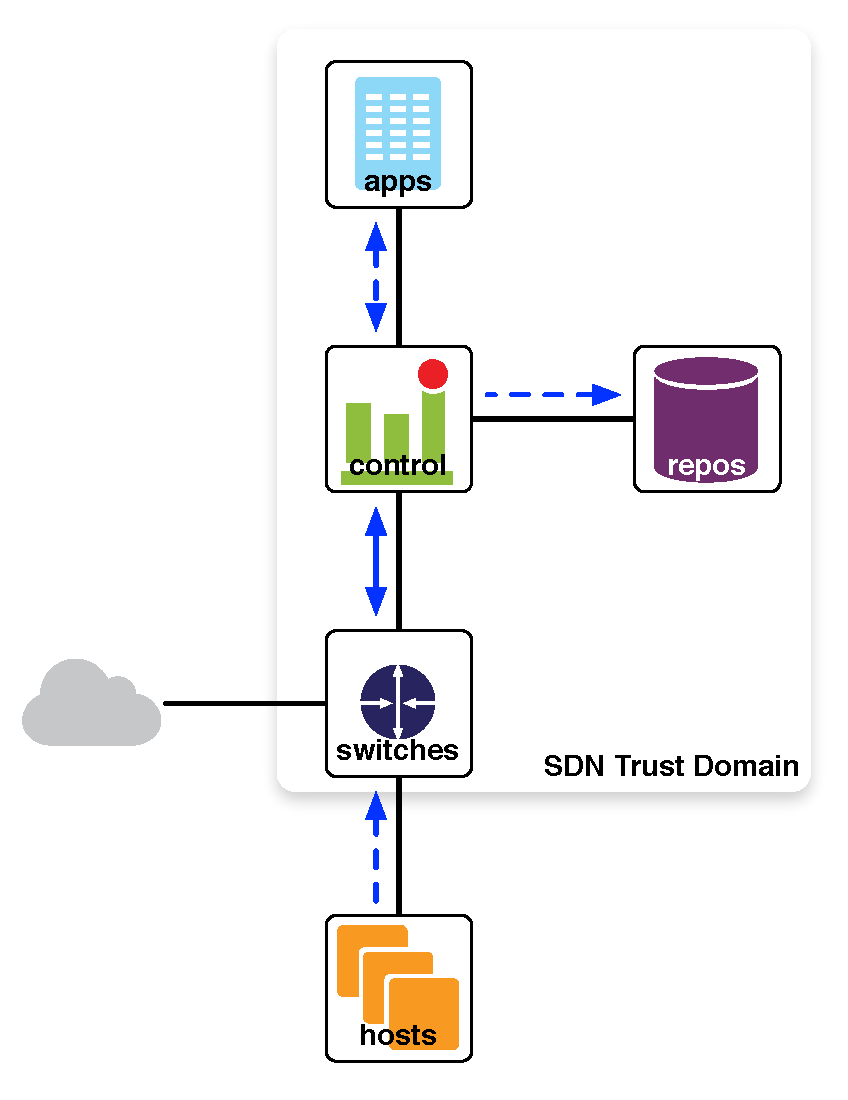
\includegraphics[width=2.5in]{images/reference-model.pdf}
\caption{A reference model for SDN based on modern systems with north- and south-bound interfaces.  Note the contextual data repositories, and the highlighted trust domain specific to SDN.}
\label{fig:reference-model}
\end{figure}

Hosts connect to {\bf switches}, which perform any number of network traffic management including routing.  Switches connect hosts to larger networks and the wider internet.  

In SDN systems, switches are controlled by {\bf controllers} that implement rules describing what flows should be allowed.  Note that in modern SDNs, all switches need not be SDN switches to enable programmable networks, but within this model we only consider SDN-enabled switches as our focus is on SDN networks and trust, not traditional non-programmable network hardware.  Controllers implement policies and host programs that process both northbound and southbound interfaces to support application and switch communication respectively.  

In order to manage networks effectively and apply defined policies appropriately, controllers need access to wider contextual information including operational state, overarching policy information, authentication data, and the like.  This information is contained in groups of {\bf repositories}, hosted in various geographic locations.  Information contained in repositories can very well be cached, though in the scope of this model we will regard repository caches as repositories as they still provide relevant and necessary information to controllers.  

Finally, we include groups of {\bf applications} that submit network management requests to various controllers.  The controllers can regard such requests as optional or required, depending on the authority of the submitting application.

All communication is over {\bf networks} of various physical types.  These networks can be wireless or wired, using virtually any protocol, though IP networks are arguably the most common realistically and originally the only supported network type~\cite{openflow1.0}.  We can use different physical networks for control plane communication or a single network for both control and data plane packets.

The next sections describe from a confidentiality, integrity, availability, non-repudiation, and authentication perspective the types of trust that components expect within a typical SDN.  The hosts and relationships outlined below follow those presented in Figure~\ref{fig:reference-model}.

\noindent
{\bf host $\leftrightarrow$ switch.} A host must be able to trust that a switch will provide flow routing services compliant to local policies.  This may or may not include respecting the confidentiality of the traffic. In some cases, like traffic in places of employment, confidentiality may not realistically be an expectation because of content monitoring or data lost prevention needs.  Integrity expectations with respect to actual traffic are high in all cases.  Certain network middleboxes may change packet header information, but should never alter data bytes within a given packet.  Availability expectations for networks overall are very high as well.  Hosts have no expectation of non-repudiation of switch services as all flow management operations are transient.  Ideally, hosts would be able to authenticate switches however without or with very little {\sl a priori} knowledge.  Also, note that these expectations are in of the entire network; the connecting switch is just representative of the network to the host.

Switches do not access services provided by hosts, and need to have very little trust if any in a given host.  They may however enforce non-repudiation with respect to individual flows or packets and users generating given flows or packets.  A typical example of this kind of requirement stems from network forensics needed after malicious insider activities. Switches may also require host and user authentication~\cite{CaFrPeLu:07}.  This kind of authentication is a prerequisite for non-repudiation, but may also be needed in networks with strict policies regarding who can connect.

\noindent
{\bf switch $\leftrightarrow$ controller.}
Switches extend a tremendous amount of trust to controllers.  Some of that trust is transitive as well, based on trust extended first to switches by attached hosts.  A switch accepts instructions on how to manage network flows from a controller.  Using OpenFlow as an example of a typical protocol between switches and controllers, controllers submit instructions either proactively or reactively to switches adding, changing, removing, or extracting flows from flow tables~\cite{openflow1.4}.  Switches have very little control over the content of these kinds of command messages beyond how they are specifically implemented.  In this environment, confidentiality of command submitted by the controller to the switch is likely not critical as these rules can be extracted from active network traffic through observation, and are furthermore constrained by known policies.  In some cases however, the content of specific commands may be best kept confidential.  Specifically, commands involving redirection of suspected malicious traffic may need to be kept confidential from other malware components that may be present.  Overall however, the effects of these commands is relatively easy to extrapolate from network traffic so keeping commands confidential may be of little real value.

Integrity and Availability, however, are much more important.  Switches need guarantees that received commands are from authenticated controllers and that the commands have been inappropriately changed en-route.  The availability of a controller for a given switch is one of the key assumptions of SDN, so controllers have stringent high-availability requirements.  Non-repudiation is important insofar as it is related to integrity and forensics.  If controllers are evaluated on commands submitted over time, maintaining a history of non-reputable commands issued by controllers becomes vital in order to avoid reputation poisoning attacks.  Authentication of controllers is vital to prevent false controller insertion.

Controllers again access no critical switch services and are correspondingly less sensitive to a lack of trustworthy switches.  Network function is clearly impacted by malicious or malfunctioning switches however.  From that perspective, the network needs to trust that the switch is implementing the commands issued by a controller.

\noindent
{\bf controller $\leftrightarrow$ repository.}
A controller is dependent on a data repository in some cases for information regarding local routing decisions.  Information delivered from these repositories should be confidential in some cases, depending on the information.  It must be delivered with integrity, however.  If controllers make decisions based on information from these repositories, adversaries tampering with delivered information can undermine the fidelity of controller decisions.  This implies that data repositories must also be authenticated.  Again, non-repudiation comes into play when trying to evaluate the reputation of a given repository for delivering valid information and for network forensics in cases where information may have been altered without authorization.  The need for highly available repositories varies based on the controller's need for information offered by a given repository.  For example, a given controller may not be able to function without authentication information describing switches, but it may be able to establish local network flows without global data describing the overall state of the larger network~\cite{ScSu:13}.

Data repositories need to authenticate controllers requesting information and may need to keep sensitive information confidential in transit.  Repositories also need to ensure information has guaranteed integrity.  The need for availability is based on information criticality, as shown previously, and non-repudiation operates under forensic constraints primarily.

\noindent
{\bf controller $\leftrightarrow$ application.}
In this case, controllers need to ensure that commands from applications have not been tampered with, are appropriate given the authorization level of the application, and that the application is authenticated.  Commands themselves need not always be confidential, nor do they need to be unable to be repudiated.  Availability of a given application is related to the application's role.

Applications, on the other hand, should be able to authenticate controllers to ensure that they are not submitting commands to rogue systems.  The commands themselves need not generally be confidential.  Communication from a controller to an application however does have strong integrity requirements to ensure that status messages are not intercepted and altered en route.  Non-repudiation again has very little functional impact.

\subsection{Overall Security Attribute Commonality}
\label{sec:commonality}
Overall, non-repudiation is generally not a high-priority security attribute in any of the trust relationships.  In all cases, it is related to forensics and reputation measures.  If designers use a reputation strategy to influence trust, non-repudiation becomes much more important.

Likewise, confidentiality tends to not be a vital attribute.  Information delivered to switches from controllers can generally be extrapolated from overall network behavior.  This becomes influenced more by the data transmitted than the relationships between entities.

Availability is of varying importance depending on the entity.  Controllers must be highly available, though switches can be less so.  Controller outages impact wide swathes of switches, while an individual switch will usually impact a smaller number of users.  Repositories and applications have availability needs lower than that of switches as controllers can operate for some period of time without direct application or repository input~\cite{ScSu:13}.

Authentication and integrity are always important.  In each trust relationship, one of the participants provides critical services, while the other provides critical data-plane management functionality.  In all cases, entities need to have confidence that the information they are given is from a credible source and the information delivered is sent to an known and authorized receiver.  They also need to have confidence that the delivered information has not been tampered with en-route.

\subsection{Differentiating Attributes of Software Defined Networks}
\label{sec:attributes}
SDNs have different behavioral and structural characteristics when compared to other systems in typical trust literature focusing on mobile ad-hoc networks (MANETs), Agent-based systems, social media, or typical e-commerce systems~\cite{ChSwCh:11,JoIsBo:07,SaSi:05,ShNePa:13,GoMo:12}.

\noindent
{\bf Limited control-plane volatility and mobility.} In MANETs, devices regularly attach and detach to running networks. Agents in agent-based systems act in a similar way, engaging in activities in an unpredictable way, though less randomly than MANET devices.

While this enables some amount of {\sl a priori} configuration of SDN controllers, switches, and the like, that configuration should be limited as much as possible to lower the cost to maintain a given SDN.  Existing approaches to SDN authentication do use approaches that require preliminary device configuration~\cite{CaFrPeLu:07}, and secure SDN designs will likely not be able to avoid this.

\noindent
{\bf Centralized high-availability.} SDNs have clear high-availability requirements with respect to controllers.  This differs from MANETs in which enrolled devices take on a variety of roles, leading to intrinsic high-availability potential.  Social and agent-based systems have wide ranges of needed availability, but in general those requirements are not intrinsic requirements necessitated by basic architectures, unlike switch dependencies on controllers.  E-commerce systems, on the other hand, have high-availability requirements distributed throughout.

This implies more distributed trust while also providing the opportunity to employ reputation or error correcting schemes over controllers.  For instance, a system could have multiple controllers deployed all of which have access to the same supporting information and can submit commands to the same switches.  The switches themselves could compare performance and flow commands between controllers, using byzantine strategies or reputation measures to detect malicious or malfunctioning controllers~\cite{FeMi:88, TaKaCh:11}.

\noindent
{\bf Clearly defined roles.} SDN control entities have clear roles, as opposed to MANETs.  In SDNs, as previously outlined, we have a variety of possible roles, ranging from controllers to switches to managing applications, with each role assigned to an individual system or system group.  MANETs are not so clearly specified --- devices in MANETs fulfill a variety of roles simultaneously, routing traffic while originating and controlling local flows.

This clear demarcation in SDN roles makes managing trust easier.  As previously shown, this has clear impacts on the kinds of security attributes given systems must exhibit.  For instance, Controllers need high-availability, while every component of a full SDN stack requires strict authentication and message integrity.

\noindent
{\bf Predictable expected behavior} As SDN entities have clearly defined roles, they should have more predictable expected behavior.  Agent-based or social systems can have very large variations in activity, depending on the range of possible agent behaviors and the extent of human involvement in social systems.  Likewise, though more constrained, devices supporting MANETs also have a larger range of possible activities resulting from the correspondingly larger number of responsibilities when compared to SDN elements.

This smaller range of possible behavior allows reputation or compromise detection systems more potential accuracy in evaluating systems.  After all, If the range of expected behavior is narrow, outlier detection is correspondingly easier.

\subsection{Promising Approaches to Trust Management}
As mentioned in section~\ref{sec:elements}, our focus is defining trust in SDN with respect to accepted security attributes like confidentiality and integrity taking into account risk, utility, and reliability of services.  We have further refined the most critical attributes in section~\ref{sec:commonality} to integrity, authentication, and availability.  Finally, in section~\ref{sec:attributes}, we described the key attributes of SDN that influence the types of implementable trust models.

Due to the more fixed nature of SDNs, we can use centralized rather than distributed systems to provide security services.  MANETs have by necessity been moving in the direction of authentication via distributed Certificate Authorities (CAs) and binary trust models, in which trust is a binary attribute to be extended in full or not extended at all~\cite{OmChBo:09}. SDNs, due to their more fixed nature, can take advantage of simpler, centralized trust schemes using PKI~\cite{Pe:99}.

Of the specific models outlined for use in PKI, the least applicable are {\sl Anarchy} or {\sl Web-of-Trust}, primarily due to scalability concerns. Other models not likely to be of much use are {\sl Relative Names}, due to a lack of industry support, and {\sl Flexible Bottom-up}, because of limited differentiation from other models (though {\sl Flexible Bottom-up} does support high availability via multiple root CAs)~\cite{Pe:99}.

With an established PKI infrastructure, we can begin to implement integrity and confidentiality within SDN.  Confidentiality is not a critical attribute of SDNs, but enabling channel integrity can supply confidentiality as a side-effect.  For example, using PKI to establish and protect control channels between switches and controllers via Transport-Layer Security (TLS) provides both channel integrity and confidentiality.  TLS is supported in OpenFlow, for example, and does provide some protection for controller traffic~\cite{openflow1.4}.

We could also begin to digitally sign flow commands issued by specific controllers, something that is not currently supported in OpenFlow or other accepted SDN standards~\cite{big_network_controller,openflow1.4}.  Signing flow commands allows guaranteed command integrity, while protecting the channel with TLS provides channel integrity, supporting security overall.  Digitally signing messages also provides forensic capabilities and the ability to track the reliability of flow commands from a specific host, leading to possible reputation metric development.

Finally, availability via the use of multiple controllers is a recent addition to the OpenFlow standard~\cite{openflow1.4}.  Switches using multiple controllers can compare flow commands, for example, enabling byzantine error correction and detection~\cite{FeMi:88, TaKaCh:11}.  This also clearly enhances controller availability.

Risk, utility, and reliability are more difficult to define in SDN and depend on all participants in a trust relationship~\cite{JoPr:04}.  For example, with respect to the relationship between a switch and a controller, the utility of the controller from the switch's perspective is clear --- the switch needs guidance from the controller with respect to establishing the correct routes for network traffic based on any number of possible parameters.  The risk to the switch for trusting a controller revolves around controllers submitting bad information to the switch.  This bad information may be flow directives that are contradictory, lead to slow traffic delivery, cause loop formation, or otherwise prohibit or retard packet delivery.  The reliability of the controller ties to the quality of the flow directives as well as quality-of-service.  Controllers with high latency are of low reliability, as are controllers that issue bad flow commands.

Overall, trust models in SDN can be centralized and take advantage of resulting simplicity.  They can furthermore take advantage of established PKI trust models with TLS and multiple controller configurations to provide more trustworthy services.  Digital signatures are however unsupported within most SDN protocols and those protocols suffer from a corresponding lack of message-level integrity as a result.  Finally, risk, utility, and reliability trust models do apply in SDN and designers can use them to more granularly define trust relationships and provide dynamic rather than binary trust between service providers and consumers.

\section{Related Work}
Trust in general has been extensively studied, with recent work on Bayesian, Fuzzy Logic, and Game Theoretic models~\cite{ChSwCh:11,JoIsBo:07,SaSi:05,ShNePa:13,GoMo:12}.  Additional techniques applied to trust modeling include trust algebras~\cite{WeCuBo:09,Jo:99} and subjective logic~\cite{JoHaPo:06,subjective_logic}.

Williamson had argued against formally defining trust, claiming that other component measures could be used more effectively without combining them into a single concept~\cite{Wi:93}.  Later, McKnight and Chervany divided trust into reliability trust and decision trust~\cite{McCh:96}, where reliability trust demonstrates that an entity trusts a third party to perform a given action, while decision trust demonstrates trust that the action will be performed correctly.  Josang and Presti extended this distinction in types of trust and derived a formal model using reliability, utility, and risk~\cite{JoPr:04}.  Trust can be alternatively classified into provision, access, delegation, identity, and contextual trust, where McKnight and Chervany's reliability and decision trust could be subclasses of Delegation trust.  Omar et. al. in 2009 presented a reliable and distributed trust model for devices in mobile networks using threshold cryptography and provided a concise survey of trust work in these networks in the process~\cite{OmChBo:09}.

With respect to SDN, Schmid et. al. outlined a formal graph theoretical approach to how network designers can incorporate local algorithms in distributed networks efficiently.  They show that while many optimization problems are easily solvable via global controllers, other non-functional requirements impose demands that can only be resolved via multiple controller schemes. They then show how link assignment and spanning tree verification can be efficiently implemented computationally by relaxing optimality requirements and accepting near-optimal solutions and implementing proof-carrying packets, respectively, introducing the idea of a {\sl supported locality model} for distributed computing \cite{ScSu:13}.  In 2012 Heller et. al. examined optimal controller placement and redundancy in modern large-scale networks. They used topologies from the Internet2~\cite{internet2} project as well as the internet topology zoo~\cite{internet-topo-zoo}. Using average and worst case optimization approaches, Heller established a property of diminishing returns with respect to the number of deployed controllers, though the specific effects of controller placement on performance varies widely based on the specific network in question.  Interestingly, given specific network performance overheads, a single controller seems to meet the performance demands of most topologies\cite{HeShMc:12}.  In 2007, Casado et. al. published their experiences with {\sl Ethane}, an early flow-based centralized controller framework to enable communication policy application over a network using both device and user authentication.  They presented and outlined not only Ethane's implementation and performance, but also a policy language {\sl POL-ETH}, for developing policies over {\sl Ethane} controlled networks.  They also outlined a group of the first fundamental principles of policy design and application over software-defined networks that can still apply today~\cite{CaFrPeLu:07}.

\section{Conclusions}
In this paper we outlined initial constraints of trust within SDNs.  We started by defining a reference model for modern SDNs based on current work.  We then defined the trust relationship between the various entities based on confidentiality, integrity, availability, non-repudiation, and authentication attributes.  We described the entities, as well as the implications of the security characteristics on those entities.  We then analyzed the differences between SDNs and other domains with active trust research, describing why those differences were important and their implications.  We closed the paper with an outline of promising approaches worthy of investigating with respect to establishing SDN trust models.

With this foundation, we will investigate the outlined approaches to dynamic and robust trust in SDN, experimentally validating promising approaches and outlining the advantages and disadvantages to the models to help guide application.  We will also add additional non-traditional security attributes like usage control to the more established list of security attributes.  Experimental validation will include simulated and as much as possible operational use to fully characterize trust model efficacy and implementability.

\printbibliography
\end{document}